\chapter{Resultados Obtidos}
\label{cap:impl}

Para realização dos testes, foram
selecionados 6 tópicos distribuídos em duas categorias diferentes, que são:
comentários políticos e comentários sobre filmes. Optou-se pela escolha de duas
categorias distintas com o objetivo de avaliar a assertividade do método
desenvolvido em diferentes contextos. Como a validação dos resultados é efetuada
de forma manual, e devido a restrições de tempo no desenvolvimento deste
trabalho, não foi possível efetuar a análise sobre mais tópicos ou categorias.

\section{Comentários Políticos}
\label{sec:pol}
Para a realização dos testes sobre um contexto de comentários políticos,
foram executados testes sobre os comentários listados abaixo e que foram
descritos Seção \ref{sec:textos}. Para tanto, foi utilizado o Método de
Propagação Dupla e a restrição da palavra alvo \textit{``Trump''}. Para a
aplicação do Método de Propagação Dupla, utilizou-se como conjuto de textos
para a expansão os próprios comentários destes tópicos.

\begin{itemize}
  \item
  \textit{Donald Trump to strip all funding from State Dept team promoting
  women's rights around the world - Leaked plan comes as First Daughter Ivanka
  defends her father's record with women}.  
  \item
  \textit{Sweden asks the U.S. to explain Trump comment on
  Sweden}.
  
  \item\textit{“Canada will welcome you,” Trudeau invites refugees as Trump bans
  them}.
\end{itemize}

Na Figura \ref{fig:pol1}, tem-se os resultados obtidos. Observa-se que
a assertividade foi próxima aos valores obtidos por Hutto e Gilbert
\cite{conf/icwsm/HuttoG14} para avaliações de produtos da Amazon e para
editoriais do New York Times. Porém, os valores foram inferiores aos obtidos na
avaliação de \textit{tweets}. 

\newpage
 
\begin{figure}[!htbp]
\centering
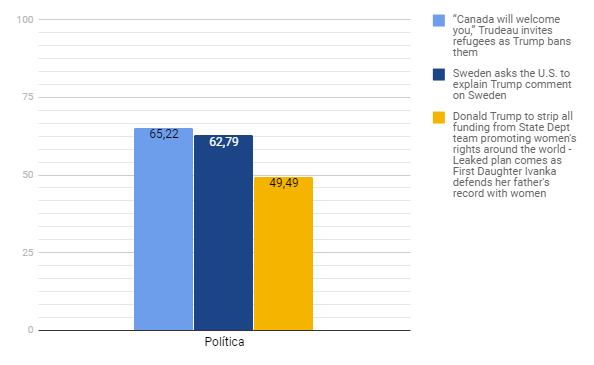
\includegraphics[height=200px]{imagens/politica1.png}
\caption{Assertividade da ferramenta desenvolvida com relação a comentários de
política.}
\label{fig:pol1}
\end{figure}

De forma a
avaliar se os resultados foram ocasionados pela diferença de contexto ou por
seus corpos de texto terem diferentes tamanhos, foi também conduzida uma análise
separando todos os comentários de política em três categorias de acordo com o
número de caracteres, que são: comentários com 144 caracteres ou menos,
similares a \textit{``tweets''}; tópicos com menos de 1000 caracteres; e tópicos
com 1000 caracteres ou mais. Na Figura \ref{fig:pol2} tem-se os resultados obtidos através da análise através da quantidade de caracteres.
Observa-se que o método apresenta uma diminuição na sua assertividade com o
aumento do texto. Essa tendência já foi observada nos
trabalhos de Hutto e Gilbert \cite{conf/icwsm/HuttoG14} onde \textit{``tweets''}
analisados apresentaram maior assertividade do que editorias do \textit{New
York Times} e as avaliações de produtos da \textit{Amazon}.


\begin{figure}[!htbp]
\centering
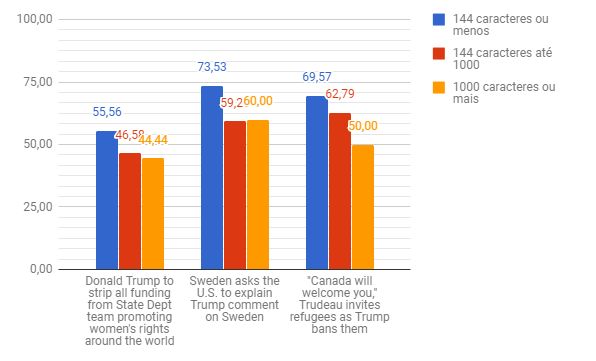
\includegraphics[height=200px]{imagens/politica2.png}
\caption{Assertividade da ferramenta desenvolvida com relação a comentários de
política por tamanho.}
\label{fig:pol2}
\end{figure}




\section{Comentários sobre Filmes}

Os mesmos testes foram realizados utilizando a palavra \textit{``movie''} como
alvo, em tópicos de cinema. O método \ac{VADER}, foi utilizado usando o método
de Propagação Dupla, sendo que os textos selecionados para a expansão e, para a
posterior análise foram obtidos dos comentários dos tópicos:

\begin{itemize}
  \item
  \textit{Official Discussion - mother! [SPOILERS]}: esse tópico contém 5297
  comentários e encontra-se disponível em
  \textit{\url{https://www.reddit.com/r/movies/comments/706y1p/official_discussion_mother_spoilers/}}
  e apresenta a avaliação do filme \textit{``Mother!''}.
  \item
  \textit{Official Discussion: Gerald's Game [SPOILERS]}: esse tópico contém 892
  comentários e
  encontra-se disponível em
  \textit{\url{https://www.reddit.com/r/movies/comments/73g2fx/official_discussion_geralds_game_spoilers/}}
  e apresenta a avaliação do filme \textit{``Gerald's Game''}.
    \item
  \textit{Official Discussion: The Mummy (2017) [SPOILERS]}: esse tópico contém
  1333 comentários e
  encontra-se disponível em
  \textit{\url{https://www.reddit.com/r/movies/comments/6g5lmo/official_discussion_the_mummy_2017_spoilers/}}
  e apresenta a avaliação do filme \textit{``The Mummy''}.
  
\end{itemize}


Na Figura \ref{fig:fil1} tem-se os resultados obtidos. Observa-se que a
assertividade também se mostra próxima aos valores obtidos por Hutto e Gilbert
\cite{conf/icwsm/HuttoG14}.Observa-se neste caso que os resultados foram
superiores aos apresentados na Seção \ref{sec:pol}. Esse aumento na
assertividade se deve ao fatos dos tópicos de filme encorajarem ao
leitor a efetuar a avaliação do filme em questão, enquanto os comentários sobre
política apresentam no conteúdo em um \textit{link} direto para a notícia
original.

\begin{figure}[!htbp]
\centering
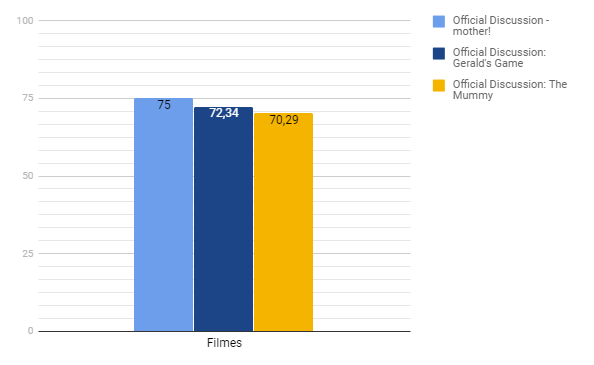
\includegraphics[height=200px]{imagens/filmes1.png}
\caption{Assertividade da ferramenta desenvolvida com relação a comentários de
filmes.}
\label{fig:fil1}
\end{figure}


Posteriormente, foi conduzida uma análise separando
os comentários de filmes, de acordo com o tamanho do texto, sendo considerados:
comentários com 144 caracteres ou menos (similares a \textit{``tweets''}), comentários com menos de 1000 caracteres e comentários com
1000 caracteres ou mais. Na Figura \ref{fig:fil2} tem-se os resultados obtidos através da
análise através da quantidade de caracteres. Observa-se que neste caso, também
houve uma queda na assertividade com o aumento do texto, como observado no
trabalho de Hutto e Gilbert \cite{conf/icwsm/HuttoG14}. 

\begin{figure}[!htbp]
\centering
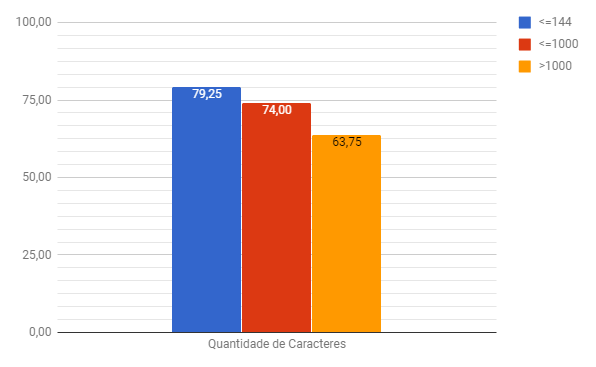
\includegraphics[height=200px]{imagens/filmes2.png}
\caption{Assertividade da ferramenta desenvolvida com relação a comentários de
filmes por tamanho.}
\label{fig:fil2}
\end{figure}
